\documentclass{article}
% s e l e c c i o n a e l t i p o de documento
\usepackage[spanish]{babel}
%
\usepackage[T1]{fontenc}
\usepackage[latin1]{inputenc}
\usepackage{graphicx}
\begin{document}
% i n i c i o d e l cuerpo d e l documento
\title{Laboratorio 1}
\author{Jean Carlos Chavarr\' ia Hughes}
\maketitle
% t i t u l o d e l documento
\begin{abstract}
Laboratorio 1 de el curso IE 0217.
\end{abstract}
\section{Introducci\' on}
Este documento corresponde al primer ejemplo desarrollado en LaTeX para el curso de estructuras abstractas de datos y algoritmos de la programaci\' on para ingenier\' ia.

\section{Respuesta a Preguntas}
\textbf{Investigue como compilar el archivo para generar como salida el archivo de extensi\' on .pdf}

Hay uan manera muy sencilla en una terminal de linux. Primero se debe tener instalado la distribucion correcta de latex, luego en el directorio donde se encuentra el documento fuente, generalmente un \textit{.tex}, se ejecuta el comando: 

\begin{verbatim}
pdflatex ejemplo.tex
\end{verbatim}

Finalmente se hace el comando

\begin{verbatim}
evince ejemplo.pdf
\end{verbatim}

\textbf{Qu\' e hace el comando branch, Y las opciones d. Qu\' e hace la opci\' on D y porqu\' e se debe tener mucho cuidado.}

En git se tiene el concepto de \textit{branch}, o rama, que es b\' asicamente un puntero sencillo que apunta a uno de los \textit{commits}. 
Por defecto, se denomina \textit{master} y cada vez que se realiza un nuevo \textit{commit}, se actualiza el puntero a apuntar el \' ultimo \textit{commit}.\\

Tal como lo menciona el manual de git, la opci\' on \textbf{-d} se encarga de 
eliminar un \textit{branch}, pero antes verifica si se encuentra completamente mezclado en su rama de subida. En cambio, el comando \textbf{-D}, no verifica el estado, si ya est\' a mezclado o no, simplemente lo elimina.\\

\textbf{Qu\' e hace la l\' inea: git checkout master.}

Esta linea de comando se encarga de regresar el \textit{master branch}.
En general, el comando \textit{checkout} se encarga de deseleccionar \textit{commits, branches and files}.

\textbf{Qu\' e hace la l\' inea: git commit -amend -reset-author}.
Esta linea b\' asicamente se encarga de evitar cometer errores con respecto al autor o el contacto utilizado al realizar un \textit{commit}, aunque en general lo que hace es reestablecer el nombre de usuario y el correo, como se puede deducir de la palabra \textit{amend}, tratar de rectificar un error.

\textbf{C\' omo recuper\' o el trabajo borrado en el repositorio de Prueba 1}

Si por accidente se elimin\' o un documento o archivo en el directorio, se puede tratar de restaurar mediante el uso del comando: 
\begin{verbatim}
git checkout --nombre_archivo.txt
\end{verbatim}
donde nombre de archivo representa el nombre del fichero eliminado.

%%
%%\textbf{¿Porqu\' e en la Prueba 2, el %%primer git status no muestra los %%cambios hechos por su compañero?}
%%
%%\textbf{¿C\' omo recupera el trabajo del %%repositorio de su compañero?}
%%

\textbf{\' Ultima parte del laboratorio}
Las cuatro partes se realizaron efectivamente, se cre\' o una cuenta en LDAP, se agrego el \textit{ssh-key} a la cuenta, se inicializ\' o el nuevo repositorio \textit{ie-0217}.



\section{Ecuaciones}
\begin{equation}
\label{etiqueta de ecuacion}
\alpha=\sqrt{\beta}
\end{equation}
\section{Figuras}
\begin{figure}[h]
\centering
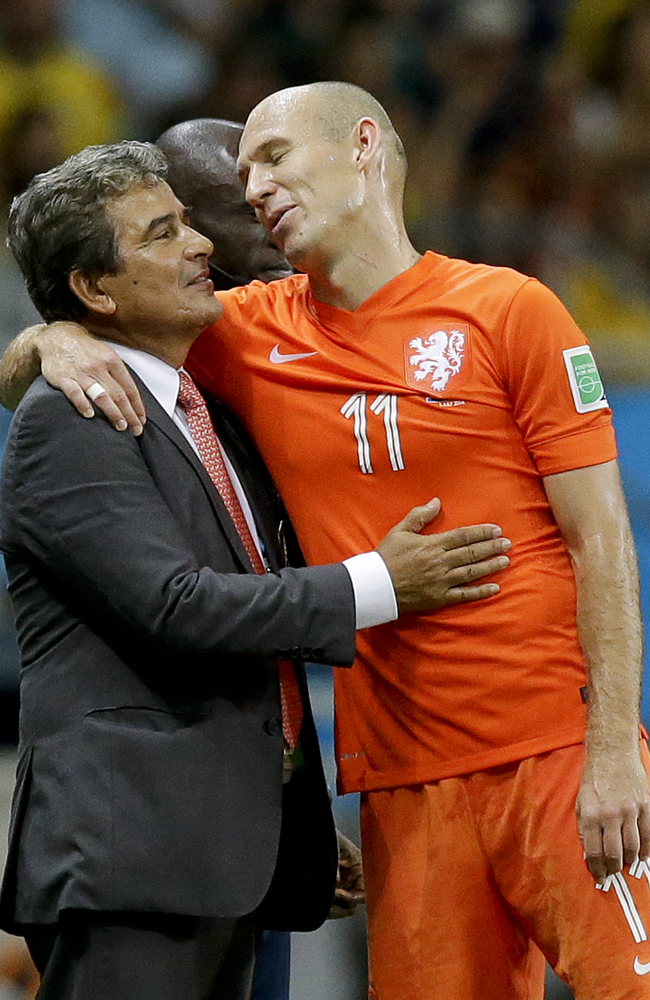
\includegraphics[width= 3.0 in]{201407051737634371468-p5.jpg}
\caption{descripcion}
\label{etiqueta_figura}
\end{figure}

\section{Tablas}

\begin{tabular} { | | l | c | r | | }

\hline
\hline

columna 1 & columna 2 & columna 3 \\

\hline

col1 & col2 & col3 \\

\hline

\end{tabular}
\end{document}
